\section{Введение}
В 1836 году Генри Фокс Талбот (Talbot) впервые наблюдал эффект, в дальнейшем названный в его честь: при прохождении монохроматического когерентного света через периодическую дифракционную решетку наблюдается повторение изображения структуры решетки на расстояниях, заданных интегральными мультипликаторами определенной длины --- длины Талбота.\\

В ходе этой работы будет рассмотрен как сам эффект, так и один из его частных случаев, интересный с практической и с эстетической точки зрения, --- ковер Талбота --- оптическая фрактальная структура. В частности, это структура используется в фотолитографии при производстве интегральных систем\cite{geinz2020}.\\

Так как наблюдение ковра Талбота в реальных условиях является затруднительным (хотя и возможно в видимом диапазоне \cite{ikonnikov2020}), в работе будут использованы искусственные модели, визуализированные с помощью Python. Мы рассмотрим способы получения данной оптической структуры с помощью методов классической и нелинейной оптики, а также способ генерации второй гармоники.\\

Весь код, используемый в работе можно найти на \href{https://github.com/aapetrakova/optics_4_sem.git}{GitHub}.\\





\section{Классический эффект Талбота}
Пусть монохроматическое волновое поле с пространственной модуляцией в плоскости, перпендикулярной направлению распространения падает на периодическую дифракционную решетку с периодом $a$, ограничимся одномерным случаем, а также гауссовым приближением, в котором можно рассмотреть преобразование луча с помощью ABCD-матрицы. Справа от экрана вследствие периодичности его структуры поле $g(x, 0)$ задано в виде суперпозиции пространственных гармоник Фурье с пространственными частотами $u_n = \dfrac{2\pi}{a}n$:
\begin{equation}
\label{1}
    g(x, 0) = \sum\limits_n c_n e^{iu_nx}
\end{equation}

Тогда поле на выходе оптической системы
\[
g(x, z) = \left(\dfrac{ik}{2\pi B}\right)^2\int g(x, 0) \cdot exp\left[\dfrac{ik}{2B}(A\xi^2 + Dx^2 - 2x\xi)\right] =
\]
\begin{equation}
\label{2}
=  A^{-0.5} exp\left[\dfrac{ikx^2}{2AB}(AD-1)\right]\cdot \sum\limits_n c_n exp\left[\dfrac{iu_nx}{A} - \dfrac{iu_n^2B}{2kA}\right]
\end{equation}

Получим решение уравнение Гельмгольца, удовлетворяющее \hyperref[1]{(2.1)}. Здесь $A$, $B$, $D$ --- элементы соответствующей ABCD-матрицы, $k$ --- волновое число, $c_n$ --- пространственный спектр.\\

Для эффекта саморепродукции необходимо, чтобы разность фаз для двух гармоник был кратен $2\pi$, так как такой набег не меняет суммарного колебания. В наших обозначениях необходимо, чтобы
\begin{equation}
\label{3}
    \dfrac{B}{A} = \dfrac{2a^2}{\lambda}n
\end{equation}

При воспроизведении изображение решетки может масштабироваться, тогда период воспроизведенного изображения
\begin{equation}
    a' = Aa
\end{equation}
Радиус кривизны волнового фронта в плоскости воспроизведения
\begin{equation}
    R' = \dfrac{AB}{AD - 1}
\end{equation}

Для наблюдения классического эффекта Талбота используется свободное пространство такое, что
\[
\begin{pmatrix}
    A & B\\
    C & D\\
\end{pmatrix} = \begin{pmatrix}
    1 & z\\
    0 & 1\\
\end{pmatrix}
\]
Тогда, подставляя в \hyperref[3]{(2.3)} значения матрицы, а также $a'$ и $R'$, получим
\begin{equation}
    z_T = \dfrac{2a^2}{\lambda}n
\end{equation}

Без ограничения общности, рассмотрим случай $n = 1$ --- первое изображение решетки, оно будет того же размера, что и сам предмет. Полученное соотношение называется длиной Талбота.\\




\subsection{Ковер Талбота}
Рассмотрим явление, наблюдаемое на расстояниях, составляющих доли от длины Талбота. Пусть $z = \alpha z_T$. Тогда
\[
g(x, z) = \sum\limits_n e^{i\dfrac{2\pi n x}{a}}e^{-i\pi n^2\alpha}
\]
Первый экспоненциальный член отвечает за сдвиг изображения, а второй за его масштабирование.

Для различных $\alpha$ получим
\begin{itemize}
    \item $z = 1/2 z_T$. Изображение сдвинется на полпериода вбок, размер останется тем же.
    \item $z = 1/4 z_T$. Видно в 2 раза больше изображений, размер уменьшен вдвое.
    \item $z = 1/8 z_T$. Видно в 4 раза больше изображений, размер уменьшен вчетверо.
\end{itemize}

\begin{figure}[H]
    \centering
    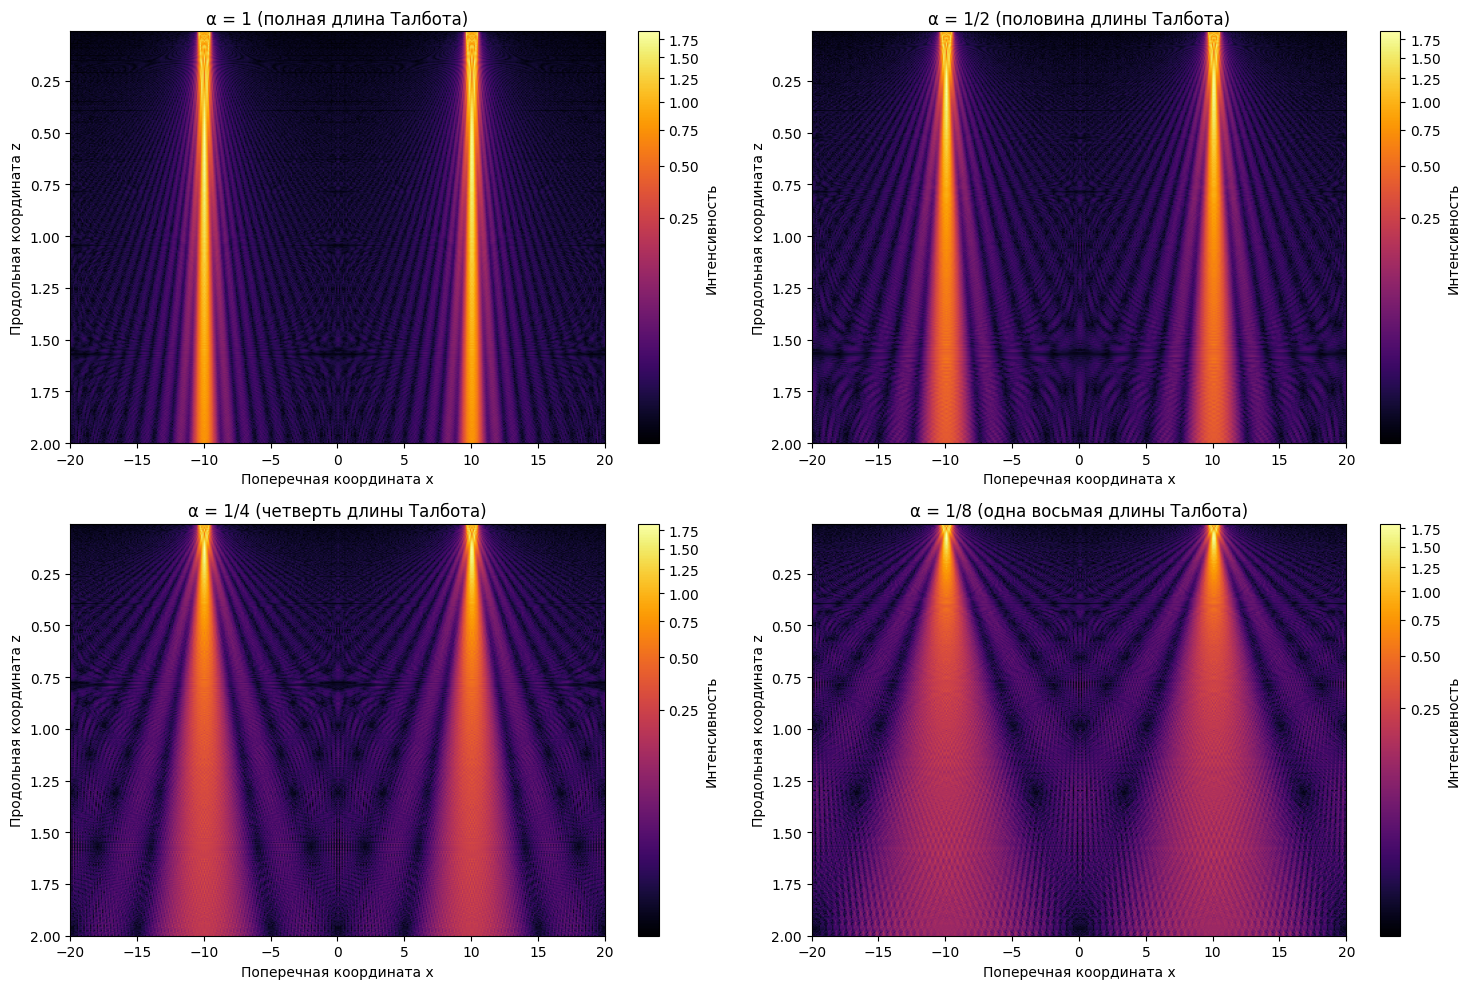
\includegraphics[width=1\linewidth]{images/распределение интенсивности.png}
    \label{I}
\end{figure}


И так далее. То есть получим фрактальную картину из сдвигающихся и уменьшающихся размеров решетки. Пример ковра Таболта показан на \hyperref[]{графике}.\\

\begin{figure}[H]
    \centering
    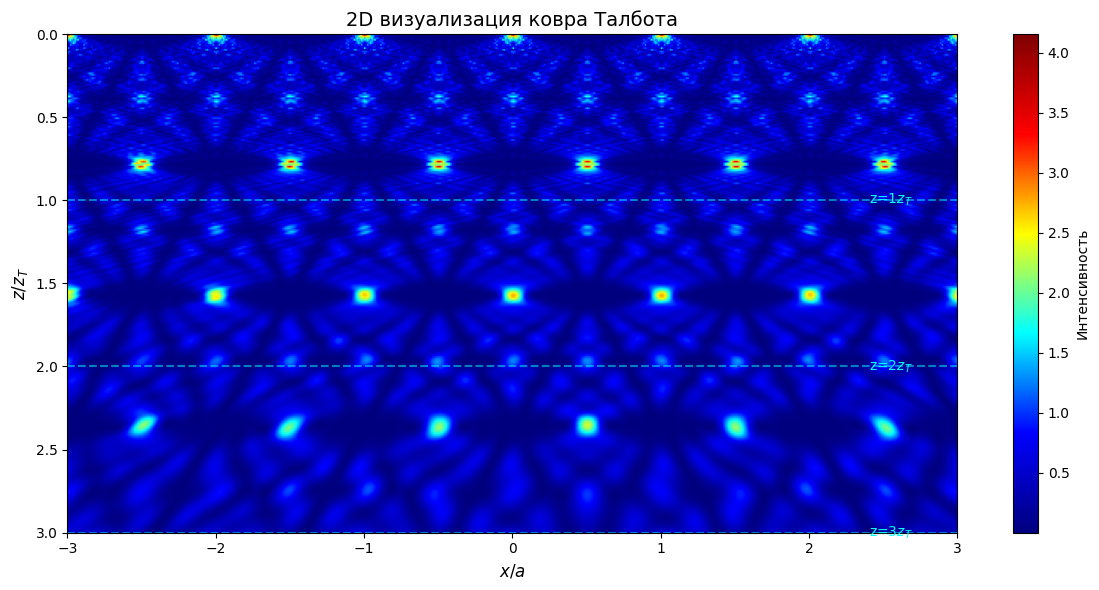
\includegraphics[width=1\linewidth]{images/2d_viz.png}
    \label{2dviz}
\end{figure}






\section{Нелинейный эффект Талбота}
Теперь рассмотрим нелинейный эффект Талбота. Как и классический эффект, нелинейный обусловлен интерференцией дифрагированных оптических пучков, но в данном случае они нелинейны, причем периодические картины интенсивности генерируемых полей на выходной поверхности нелинейных материалов могут быть восстановлены после распространения на расстояния, кратные определенному продольному расстоянию.\\

Данный процесс можно разделить на два подпроцесса.
\begin{enumerate}
    \item Нелинейный процесс внутри материала. 
    \item Свободное распространение полученного нелинейного оптического эффекта.
\end{enumerate}
Для простоты разберем генерацию только второй гармоники в одноосном нелинейном кристалле в случае отсутствия дополнительной пространственной фазы для иллюстрации эффекта.\\



\subsection{Генерация второй гармоники}


Считаем, что и падающий пучок (вдоль $z$), и генерируемый являются пространственно когерентными с равномерным распределением амплитуды и интенсивности, т.е. считаем пучки гауссовскими. Тогда плоскость максимальной интенсивности (минимальной перетяжки) пучка  находится вблизи поверхности кристалла, обозначим радиус минимальной перетяжки $w_0$. Сам эксперимент\cite{wen2011} выглядит следующим образом: пучок накачки с длиной волны $\lambda_p$ падает на одноосный кристалл, а сама интерференционная картина сгенерированной второй гармоники с длиной волны $\lambda_s$ и волновым числом $k_s = \dfrac{2\pi}{\lambda_s}$ фиксируется с помощью  CCD-камеры на определенных расстояниях $z$.\\

Опять воспользуемся приближением Френеля. Тогда поле $g(\textbf{R})$ определяется через интеграл Френеля с помощью поля когерентного источника $g_s(\textbf{r}_s)$ и функции пропускания $T(\textbf{r})$, где векторы \textbf{R}, \textbf{r}, $\textbf{r}_s$
 находятся соответственно в плоскостях наблюдения $(X, Y)$, объекта $(x, y)$ и источника $(x_s, y_s)$. В параксиальном приближении получаем:

\begin{equation}
g(\textbf{R}) = \frac{e^{ik(d_1+d_2)}}{i\lambda d_1 d_2} \int dr_s f_s(\textbf{r}_s) \int dr T(\textbf{r}) e^{ik|\textbf{r}-\textbf{r}_s|^2/(2d_1)} e^{ik|\textbf{R}-\textbf{r}|^2/(2d_2)}
\end{equation}
Здесь $d_1$ --- расстояние от источника до объекта, а $d_2$ --- от объекта до плоскости наблюдения. Так как исходная вона направлена вдоль оси $z$, вторая гармоника внутри среды хорошо описывается нелинейной оптикой и не имеет прямой связи с саморепродукцией (первый подпроцесс), а значит, при дальнейшем анализе можем сосредоточиться только на распространении этой волны от выхода из кристалла до плоскости наблюдения, что ведет к возникновению эффекта Талбота (второй подпроцесс).\\

Без дополнительной к полю второй гармоники фазы на расстоянии $z$ от выходной поверхности кристалла получим поле гауссова пучка $g_G$, предполагая некоторую однородность источника:

\begin{equation}
\label{3_2}
g_G(X,Y,z) \propto \iint dxdy\, e^{-(x^2+y^2)/w^2} T(x,y) e^{ik_s\left[z + \frac{X^2+Y^2}{2z} - \frac{xX+yY}{z} + \frac{x^2+y^2}{2z}\right]},
\end{equation}
где $w$ --- радиус гауссова пучка в произвольной плоскости, а границу нелинейного материала считаем бесконечной. В уравнении \hyperref[3_2]{(3.2)} функция пропускания для периодического объекта может быть представлена в виде ряда Фурье

\begin{equation}
T(x) = \sum_{n=-\infty}^{+\infty} b_n e^{2\pi inx/a},
\end{equation}
где $b_n$ --- амплитуда $n-$ой волны.\\

При подстановке интеграла Гаусса, уравнение \hyperref[3_2]{(3.2)} принимает вид

\begin{equation}
\label{3_4}
g_G(X,Y,z) \propto A_0 e^{-k_s^2(X^2+Y^2)/(4\alpha z^2)} \sum_{n=-\infty}^{+\infty} b_n e^{-\pi^2 n^2/(\alpha a^2)} e^{\pi n k_s X/(\alpha a z)}
\end{equation}

где $\alpha = 1/w^2 - i k_s/(2z)$, более того, $\alpha$ можно связать с радиусом перетяжки SH-пятна как 
\[
|\alpha|^2 = \left(\dfrac{w_z}{w_0}\right)^2,
\]
где $w_z = w_0\sqrt{1 + (2z/_sw_0^2)^2}$ --- радиус пучка в плоскости наблюдения.\\

В дальнейшем не будем учитывать экспоненциальный член перед знаком суммирования в \hyperref[3_4]{(3.4)}, так как он влияет лишь на интенсивность, но не на саморепродукцию. Тогда в терминах радиуса перетяжки запишем
\begin{equation}
\label{3_5}
    g_G(X, Y, z) \propto \sum_{n=-\infty}^{+\infty} b_n exp\left[-\dfrac{n^2\lambda_s^2w_0^2z^2}{a^2w_z^2}\right] exp\left[\dfrac{2n\lambda_sw_0^2zX}{aw_z^4}\right] exp\left[-i\dfrac{\pi\lambda_sn^2w_0^2z}{a^2w_z^2}\right] exp\left[i\dfrac{2\pi n w_0^2X}{aw_z^2}\right]
\end{equation}
Первые два экспоненциальных члена не участвуют в самовоспроизведении, поэтому не будем учитывать их далее.\\

\begin{equation}
e^{-i\pi \lambda_s n^2 w_0^2 z/(a^2 w_z^2)}
\end{equation}
--- локализационный член, так как он описывает изменение фаз, а значит, приравняв его к $2\pi$ получим длину Талбота в нелинейном случае:

\begin{equation}
z'_T = 2m \left(\frac{a^2}{\lambda_s}\right) \left(\frac{w_z}{w_0}\right)^2,
\end{equation}
где $m\in \mathbb{N}$ --- число саморепродукции. Когда $m$ --- нечетное, изображение сдвигается на полпериода относительно объекта.\\

Последний же экспоненциальный член в уравнении \hyperref[3_5]{(3.5)} отвечает за поперечное увеличение дифракционной картины:

\begin{equation}
M_G = \left(\frac{w_z}{w_0}\right)^2
\end{equation}


\subsection{Ковер Талбота в нелинейном случае}
В связи с выкладками выше, можем утверждать, что на расстояниях $0 < z < z'_T$ вновь будет наблюдаться ковер Талбота, отличие в значениях сдвигов относительно изображения на одной длине Талбота и увеличении воспроизведенного изображения.\\

\begin{figure}[H]
    \centering
    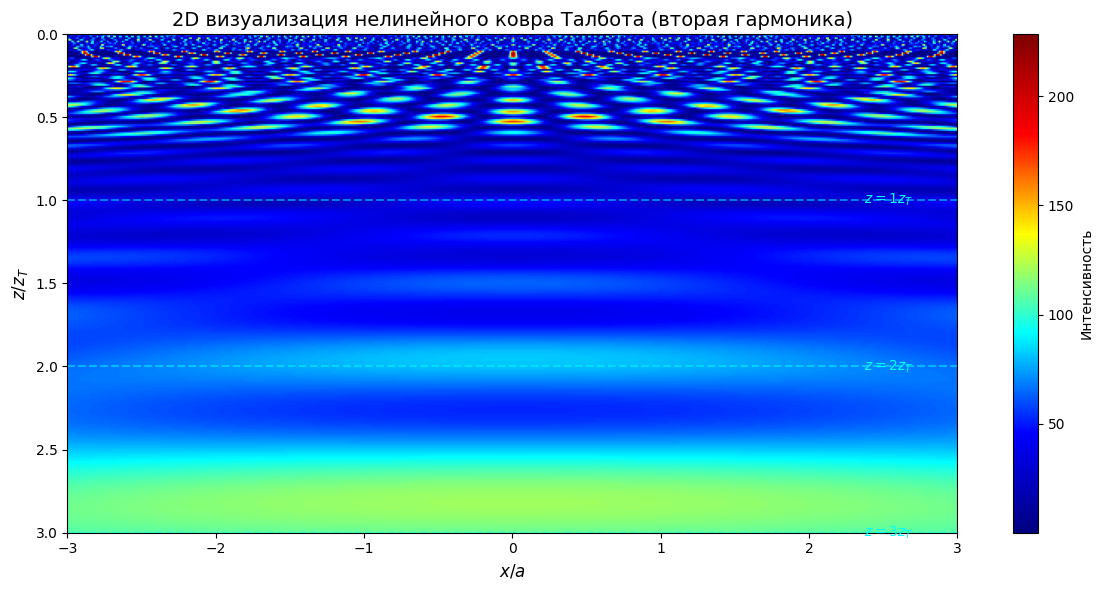
\includegraphics[width=1\linewidth]{images/sh.png}
    \label{sh}
\end{figure}













\begin{thebibliography}{99}

\bibitem{geinz2020}
Гейнц Ю.Э., Землянов А.А., Панина Е.К., Минин И.В., Минин О.В.
\newblock Получение высококонтрастных «ковров Талбота» при использовании амплитудно-фазовой мезоволновой маски.
\newblock \emph{Оптика атмосферы и океана}, 33(8): 656--663, 2020.\\
% где ты гптшила код?
\newblock DOI: \href{https://doi.org/10.15372/AOO20200810}{10.15372/AOO20200810}.

\bibitem{ikonnikov2020}
Ikonnikov, D.A., Myslivets, S.A., Volochaev, M.N. et al.
\newblock Two-dimensional Talbot effect of the optical vortices and their spatial evolution. 
\newblock \emph{Scientific Reports} 10, 20315 (2020).\\
\newblock DOI: \href{https://doi.org/10.1038/s41598-020-77418-y}{10.1038/s41598-020-77418-y}

\bibitem{}
Кандидов В.П., Кондратьев А.В.
\newblock Эффект Таьбо в гауссовых оптических системах\\
\newblock \emph{Квантовая электроника}, 2001, том 31, номер 11, 1032-1034

\bibitem{wen2011}
Wen J., Zhang Y., Zhu S.-N., Xiao M.
\newblock Theory of nonlinear Talbot effect\\
\newblock \emph{Optics Letters}, 2011. — Vol. 28, No. 2. — P. 275--280.

\bibitem{cruz2020}
Cruz-Félix, A.S., Martínez-Niconoff, G., Alvarado, A.S., Sánchez Hernández, H.H., Ramírez-San-Juan, J.C.
\newblock Coherent-mode representation of self-imaging optical fields.
\newblock \emph{Optik}, 203, 164016, 2020.

\bibitem{ikonnikov2021}
Ikonnikov, D.A., Myslivets, S.A., Arkhipkin, V.G., Vyunishev, A.M.
\newblock 3D Optical Vortex Lattices.
\newblock \emph{Annalen der Physik}, 533, 2100114, 2021.


\bibitem{sbitnev2009}
Сбитнев В.И.
\newblock Интерференционные явления: фракталы в ближней зоне, Талбот-ковры и поведение бомовских траекторий на них.
\newblock \emph{Квантовая Магия}, 6(4): 4155--4168, 2009.


\end{thebibliography}
